\section{Determinación de subredes}
A partir de la topología entregada y el espacio de direccionamiento asignado, se procedió a realizar el \textit{subnetting} de la red. El espacio 
de direccionamiento asignado es el mostrado en la tabla \ref{tab001}. La resolución de direcciones asignadas que se realizó siguiendo el estandar
esbozado en el \textit{RFC 950} se muestra en la tabla \ref{tab002}. La determinación de las redes y el nombre asociado a cada una se muestra en 
la figura \ref{fig001}. \\

\begin{table}[!htpb]
	\centering
	\begin{tabular}{|c|c|c|c|c|}
		\hline
		Tipo de Red & Dirección de Red & Máscara de Red & Red Privada & Detalles \\
		\hline
		C & 192.168.25.0 & 255.255.255.0 & Si & - \\
		\hline
		A & 10.111.25.0 & 255.255.255.0 & Si & - \\
		\hline
		B & 157.63.5.0 & 255.255.255.0 & No & Internet \\
		\hline
		A & 10.7.5.64 & 255.255.255.192 & Si & Frame Relay \\
		\hline
		A & 10.61.5.0 & 255.255.255.0 & Si & - \\
		\hline
		A & 10.61.6.128 & 255.255.255.128 & Si & - \\
		\hline
		A & 10.61.7.128 & 255.255.255.128 & Si & - \\
		\hline
	\end{tabular}
	\caption{Redes asignadas}
	\label{tab001}
\end{table}
		
\begin{table}[!htbp]
  \begin{tabular}{|c|c|c|c|c|c|c|}
    \hline
	Nombre & Incluye & \#Host & \#Routers & Total & Bloque & Dirección de red \\ \hline
	Amapola & Web Server & 240 & 4 & 244 & 256 & 192.168.25.0/24 \\ \hline
	Begonia & ~ & 29 & 3 & 32 & 64 & 10.111.25.192/26 \\ \hline
	Clavel & Telnet Server & 250 & 2 & 252 & 256 & 10.61.5.0/24 \\ \hline
	Dalia & ~ & 16 & 2 & 18 & 32 & 10.111.25.128/27 \\ \hline
	Espuela & Telnet Server & 17 & 3 & 20 & 32 & 10.61.6.128/27 \\ \hline
	Fresia & ~ & 9 & 4 & 13 & 16 & 10.111.25.160/28 \\ \hline
	Geranio & FTP Server & 124 & 1 & 125 & 128 & 10.111.25.0/25 \\ \hline
	Hortensia & ~ & 120 & 4 & 124 & 128 & 10.61.7.128/25 \\ \hline
	Iris & ~ & 8 & 2 & 10 & 16 & 10.111.25.176/28 \\ \hline
	Jazmín & ~ & 7 & 1 & 8 & 16 & 10.61.6.160/28 \\ \hline
	Kentia & Internet & 0 & 2 & 2 & 4 & 157.63.5.0/30 \\ \hline
	Lirio & ~ & 24 & 3 & 27 & 32 & 10.61.6.192/27 \\ \hline
	Margarita & PPP & 0 & 2 & 2 & 4 & 10.61.6.176/30 \\ \hline
	Narciso & PPP & 0 & 2 & 2 & 4 & 10.61.6.180/30 \\ \hline
	Orquídea & FR – R1/R8 & 0 & 2 & 2 & 4 & 10.7.5.64/30 \\ \hline
	Petunia & FR – R1/R9 & 0 & 2 & 2 & 4 & 10.7.5.68/30 \\ \hline
	Quimonant & FR – R1/R15 & 0 & 2 & 2 & 4 & 10.7.5.72/30 \\ \hline
	Rosa & FR – R8/R9 & 0 & 2 & 2 & 4 & 10.7.5.76/30 \\ \hline
	Siempreviva & FR – R8/R15 & 0 & 2 & 2 & 4 & 10.7.5.80/30 \\ \hline
	Tulipán & FR – R9/R15 & 0 & 2 & 2 & 4 & 10.7.5.84/30 \\ \hline
	Ulmaria & Internet & 0 & 2 & 2 & 4 & 157.63.5.4/30 \\ \hline
	Violeta & Tunnel & 0 & 2 & 2 & 4 & 10.61.6.184/30 \\	
    \hline
  \end{tabular}
  \captionof{table}{Tabla de asignación de redes}
	\label{tab002}
\end{table}

\begin{figure}[!htpb]
      \centering
      \begin{center}
      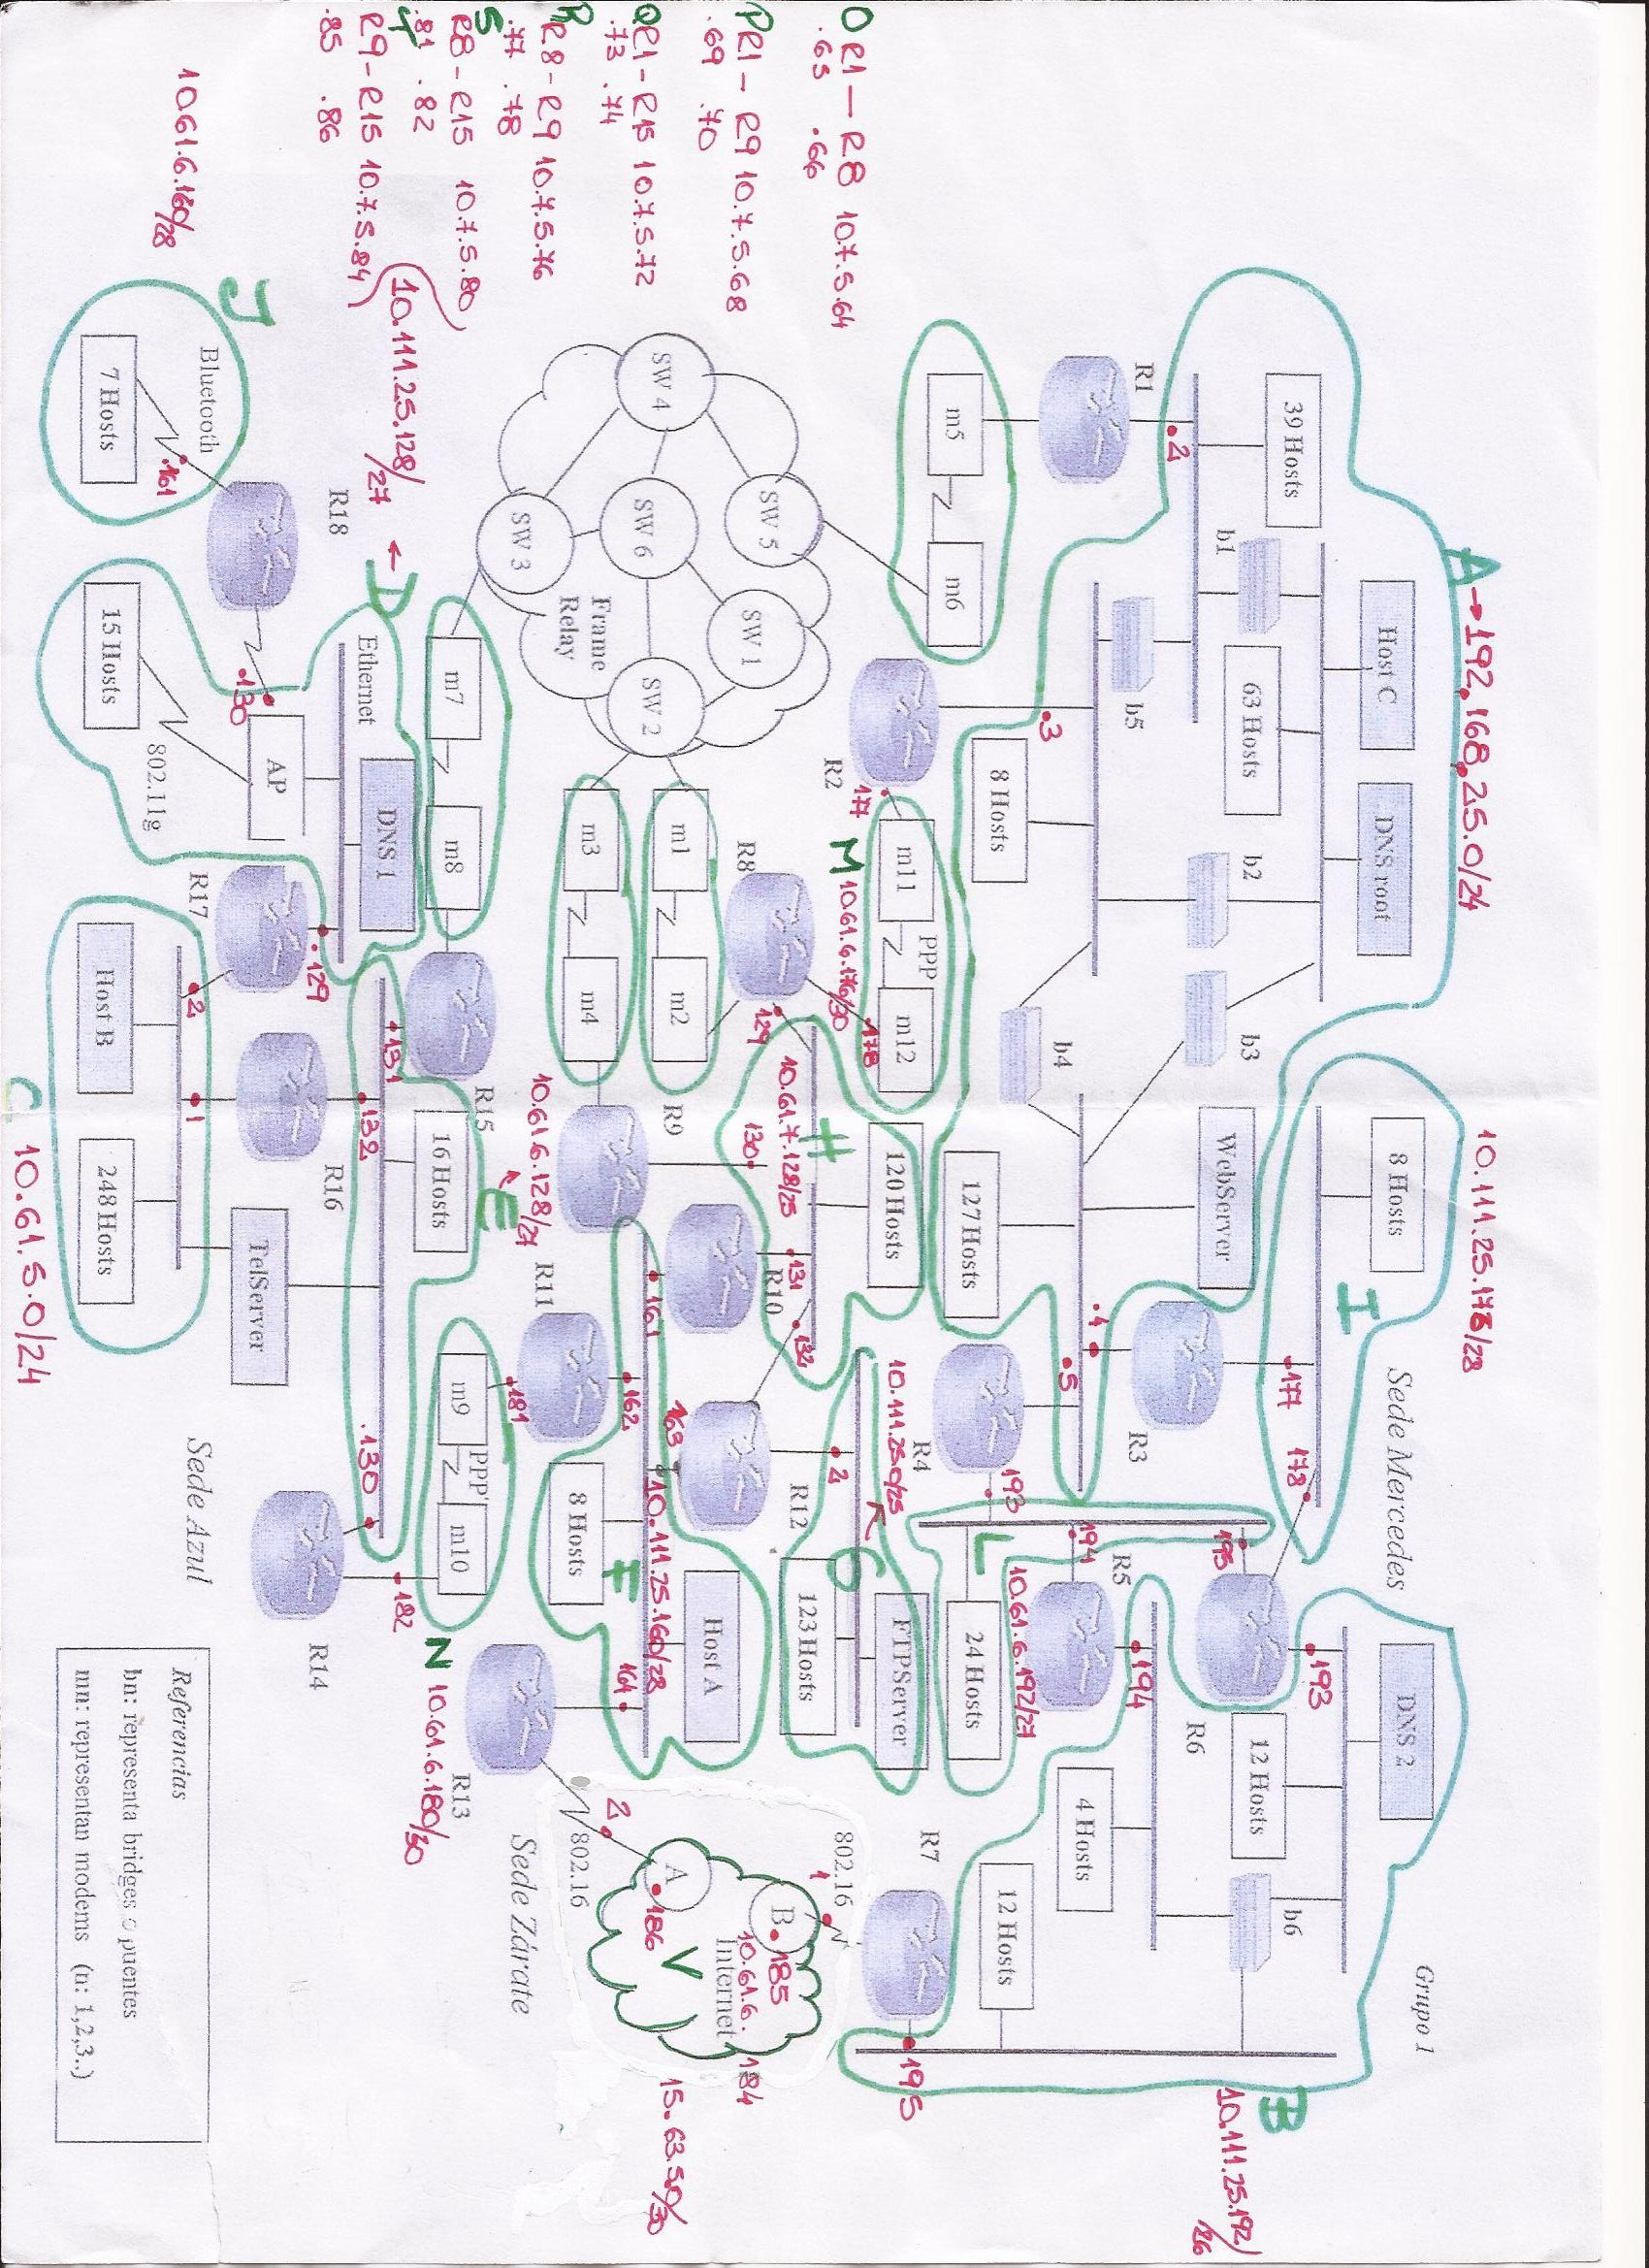
\includegraphics[width=13cm]{Imagenes/red.jpg}
      \end{center}
      \captionof{figure}{Diagrama de asignación de redes}
      \label{fig001}
\end{figure}

\begin{figure}[H]
      \centering
      \begin{center}
      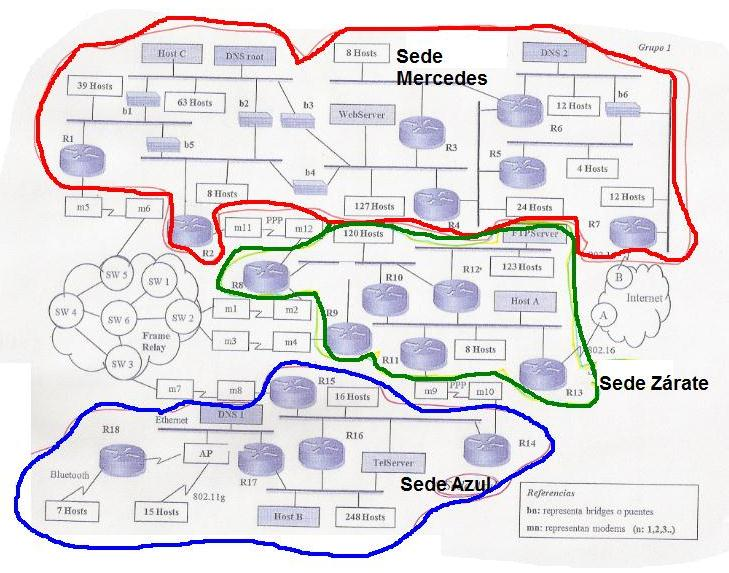
\includegraphics[width=1.2\textwidth]{Imagenes/sedes.jpg}
      \end{center}
      \captionof{figure}{Diagrama de delimitación de sedes}
      \label{fig002}
\end{figure}


La topología se divide en tres sedes: \textit{Azul, Mercedes y Zárate}. Es importante delimitar que redes pertenecen a cada sede
dado que de esto depende la resolución de nombres de dominios (DNS) y la aplicación de los protocolos de ruteo. En la figura \ref{fig002} se muestra 
la división de la red en las tres respectivas sedes. \\
\indent Con el espacio de direccionamiento asignado a cada red, se procedió a asignar las direcciones correspondientes a cada host perteneciente a las mismas. 
Las direcciones asignadas corresponden a las interfaces de los routers pertenecientes a la red y a los hosts especiales que se asignaron a las mismas
en la topología (Servers, DNSs o Hosts particulares). \\ 

\subsection{Amapola}

\textbf{Dirección de red:} 192.168.25.0/24

\begin{table}[!htbp]
\centering
  \begin{tabular}{|c|c|c|}
    \hline
	Router & Dirección & Dirección Virtual\\ \hline
	R1 & 192.168.25.2 &  - \\ \hline
	R2 & 192.168.25.3 &  - \\ \hline
	R3 & 192.168.25.4 & 192.168.25.6 \\ \hline
	R3 & 192.168.25.5 & 192.168.25.6 \\
    \hline
  \end{tabular}
  \captionof{table}{Tabla de asignación de routers en Amapola}
\end{table}

\begin{table}[!htbp]
\centering
  \begin{tabular}{|c|c|}
    \hline
	DNS Root & 192.168.25.7 \\ \hline
	Host C & 192.168.25.6 \\ \hline
	Web Server & 192.168.25.1 \\
    \hline
  \end{tabular}
  \captionof{table}{Tabla de asignaciones especiales de Amapola}
\end{table}

\subsection{Begonia}

\textbf{Dirección de red:} 10.111.25.192/26

\begin{table}[!htbp]
\centering
  \begin{tabular}{|c|c|c|}
    \hline
	Router & Dirección & Dirección Virtual\\ \hline
	R6 & 10.111.25.193 & 10.111.25.196 \\ \hline
	R7 & 10.111.25.194 & 10.111.25.196  \\ \hline
	R8 & 10.111.25.195 & - \\
    \hline
  \end{tabular}
  \captionof{table}{Tabla de asignación de routers en Begonia}
\end{table}

\begin{table}[!htbp]
\centering
  \begin{tabular}{|c|c|}
    \hline
	DNS2& 10.111.25.196 \\
    \hline
  \end{tabular}
  \captionof{table}{Tabla de asignaciones especiales de Begonia}
\end{table}

\subsection{Clavel}
\textbf{Dirección de red:} 10.61.5.0/24
\begin{table}[!htbp]
\centering
  \begin{tabular}{|c|c|}
    \hline
	Router & Dirección\\ \hline
	R16 & 10.61.5.1 \\ \hline
	R17 & 10.61.5.2 \\
    \hline
  \end{tabular}
  \captionof{table}{Tabla de asignación de routers en Clavel}
\end{table}

\begin{table}[!htbp]
\centering
  \begin{tabular}{|c|c|}
    \hline
	TelServer& 10.61.5.130 \\
    \hline
  \end{tabular}
  \captionof{table}{Tabla de asignaciones especiales de Clavel}
\end{table}

\subsection{Dalia}
\textbf{Dirección de red:} 10.111.25.128/27
\begin{table}[!htbp]
\centering
  \begin{tabular}{|c|c|}
    \hline
	Router & Dirección\\ \hline
	R17 & 10.111.25.129\\ \hline
	R18 & 10.111.25.130\\
    \hline
  \end{tabular}
  \captionof{table}{Tabla de asignación de routers en Dalia}
\end{table}

\begin{table}[!htbp]
\centering
  \begin{tabular}{|c|c|}
    \hline
	DNS1& 10.111.25.131 \\
    \hline
  \end{tabular}
  \captionof{table}{Tabla de asignaciones especiales de Dalia}
\end{table}

\subsection{Espuela}
\textbf{Dirección de red:} 10.61.6.128/27
\begin{table}[!htbp]
\centering
  \begin{tabular}{|c|c|}
    \hline
	Router & Dirección\\ \hline
	R14 & 10.61.6.130\\ \hline
	R15 & 10.61.6.131\\ \hline
	R16 & 10.61.6.132\\
    \hline
  \end{tabular}
  \captionof{table}{Tabla de asignación de routers en Espuela}
\end{table}

\begin{table}[!htbp]
\centering
  \begin{tabular}{|c|c|}
    \hline
	TelnetServer& 10.61.6.129 \\
    \hline
  \end{tabular}
  \captionof{table}{Tabla de asignaciones especiales de Espuela}
\end{table}

\subsection{Fresia}
\textbf{Dirección de red:} 10.111.25.160/28
\begin{table}[!htbp]
\centering
  \begin{tabular}{|c|c|}
    \hline
	Router & Dirección\\ \hline
	R10 & 10.111.25.161\\ \hline
	R11 & 10.111.25.162\\ \hline
	R12 & 10.111.25.163\\ \hline
	R13 & 10.111.25.164\\
    \hline
  \end{tabular}
  \captionof{table}{Tabla de asignación de routers en Fresia}
\end{table}

\begin{table}[!htbp]
\centering
  \begin{tabular}{|c|c|}
    \hline
	Host A&10.111.25.165\\
    \hline
  \end{tabular}
  \captionof{table}{Tabla de asignaciones especiales de Fresia}
\end{table}


\subsection{Geranio}
\textbf{Dirección de red:} 10.111.25.0/25
\begin{table}[!htbp]
\centering
  \begin{tabular}{|c|c|}
    \hline
	Router & Dirección\\ \hline
	R12 & 10.111.25.2\\
    \hline
  \end{tabular}
  \captionof{table}{Tabla de asignación de routers en Geranio}
\end{table}

\begin{table}[!htbp]
\centering
  \begin{tabular}{|c|c|}
    \hline
	FTP Server& 10.111.25.1\\
    \hline
  \end{tabular}
  \captionof{table}{Tabla de asignaciones especiales de Geranio}
\end{table}

\subsection{Hortensia}
\textbf{Dirección de red:} 10.61.7.128/25
\begin{table}[!htbp]
\centering
  \begin{tabular}{|c|c|}
    \hline
	Router & Dirección\\ \hline
	R8 & 10.61.7.129\\ \hline
	R9 & 10.61.7.130\\ \hline
	R10 & 10.61.7.131\\ \hline
	R12 & 10.61.7.132\\
    \hline
  \end{tabular}
  \captionof{table}{Tabla de asignación de routers en Hortensia}
\end{table}

\begin{table}[!htbp]
\centering
  \begin{tabular}{|c|c|}
    \hline
	TelnetServer& 10.61.6.129 \\
    \hline
  \end{tabular}
  \captionof{table}{Tabla de asignaciones especiales de Hortensia}
\end{table}

\subsection{Iris}
\textbf{Dirección de red:} 10.111.25.176/28
\begin{table}[!htbp]
\centering
  \begin{tabular}{|c|c|}
    \hline
	Router & Dirección\\ \hline
	R3 & 10.111.25.177\\ \hline
	R6 & 10.111.25.178\\
    \hline
  \end{tabular}
  \captionof{table}{Tabla de asignación de routers en Iris}
\end{table}

\subsection{Jazmín}
\textbf{Dirección de red:} 10.61.6.160/28
\begin{table}[!htbp]
\centering
  \begin{tabular}{|c|c|}
    \hline
	Router & Dirección\\ \hline
	R18 & 10.61.6.161\\
    \hline
  \end{tabular}
  \captionof{table}{Tabla de asignación de routers en Jazmín}
\end{table}

\subsection{Kentia}
\textbf{Dirección de red:} 157.63.5.0/30	
\begin{table}[!htbp]
\centering
  \begin{tabular}{|c|c|}
    \hline
	Router & Dirección\\ \hline
	R7 & 157.63.5.1\\ 
    \hline
  \end{tabular}
  \captionof{table}{Tabla de asignación de routers en Kentia}
\end{table}

\begin{table}[!htbp]
\centering
  \begin{tabular}{|c|c|}
    \hline
	Internet& 157.63.5.2 \\
    \hline
  \end{tabular}
  \captionof{table}{Tabla de asignaciones especiales de Kentia}
\end{table}

\subsection{Lirio}

\textbf{Dirección de red:} 10.61.6.192/27

\begin{table}[!htbp]
\centering
  \begin{tabular}{|c|c|c|}
    \hline
	Router & Dirección & Dirección Virtual\\ \hline
	R4 & 10.61.6.193 &  - \\ \hline
	R5 & 10.61.6.194 & 10.61.6.196  \\ \hline
	R6 & 10.61.6.195 & 10.61.6.196 \\
    \hline
  \end{tabular}
  \captionof{table}{Tabla de asignación de routers en Lirio}
\end{table}

\subsection{Margarita}
\textbf{Dirección de red:} 10.61.6.176/30
\begin{table}[!htbp]
\centering
  \begin{tabular}{|c|c|}
    \hline
	Router & Dirección\\ \hline
	R2 & 10.61.6.177\\ \hline
	R8 & 10.61.6.178\\
    \hline
  \end{tabular}
  \captionof{table}{Tabla de asignación de routers en Margarita}
\end{table}

\subsection{Narciso}
\textbf{Dirección de red:} 10.61.6.180/30
\begin{table}[!htbp]
\centering
  \begin{tabular}{|c|c|}
    \hline
	Router & Dirección\\ \hline
	R11 & 10.61.6.181\\ \hline
	R14 & 10.61.6.182\\
    \hline
  \end{tabular}
  \captionof{table}{Tabla de asignación de routers en Narciso}
\end{table}

\subsection{Orquídea}
\textbf{Dirección de red:} 10.7.5.64/30
\begin{table}[!htbp]
\centering
  \begin{tabular}{|c|c|}
    \hline
	Router & Dirección\\ \hline
	R1 & 10.7.5.65\\ \hline
	R8 &10.7.5.66\\
    \hline
  \end{tabular}
  \captionof{table}{Tabla de asignación de routers en Orquídea}
\end{table}

\subsection{Petunia}
\textbf{Dirección de red:} 10.7.5.68/30
\begin{table}[!htbp]
\centering
  \begin{tabular}{|c|c|}
    \hline
	Router & Dirección\\ \hline
	R1 &10.7.5.69\\ \hline
	R9 &10.7.5.70\\
    \hline
  \end{tabular}
  \captionof{table}{Tabla de asignación de routers en Petunia}
\end{table}

\subsection{Quimonant}
\textbf{Dirección de red:} 10.7.5.72/30
\begin{table}[!htbp]
\centering
  \begin{tabular}{|c|c|}
    \hline
	Router & Dirección\\ \hline
	R1 &10.7.5.73\\ \hline
	R15 &10.7.5.74\\
    \hline
  \end{tabular}
  \captionof{table}{Tabla de asignación de routers en Quimonant}
\end{table}

\subsection{Rosa}
\textbf{Dirección de red:} 10.7.5.76/30
\begin{table}[!htbp]
\centering
  \begin{tabular}{|c|c|}
    \hline
	Router & Dirección\\ \hline
	R8 &10.7.5.77\\ \hline
	R9 &10.7.5.78\\
    \hline
  \end{tabular}
  \captionof{table}{Tabla de asignación de routers en Rosa}
\end{table}


\subsection{Siempreviva}
\textbf{Dirección de red:} 10.7.5.80/30
\begin{table}[!htbp]
\centering
  \begin{tabular}{|c|c|}
    \hline
	Router & Dirección\\ \hline
	R8 &10.7.5.81\\ \hline
	R15 &10.7.5.82\\
    \hline
  \end{tabular}
  \captionof{table}{Tabla de asignación de routers en Siempreviva}
\end{table}

\subsection{Tulipán}
\textbf{Dirección de red:} 10.7.5.84/30
\begin{table}[!htbp]
\centering
  \begin{tabular}{|c|c|}
    \hline
	Router & Dirección\\ \hline
	R9 &10.7.5.85\\ \hline
	R15 &10.7.5.86\\
    \hline
  \end{tabular}
  \captionof{table}{Tabla de asignación de routers en Tulipán}
\end{table}

\subsection{Ulmaria}
\textbf{Dirección de red:} 157.63.5.4/30	
\begin{table}[!htbp]
\centering
  \begin{tabular}{|c|c|}
    \hline
	Router & Dirección\\ \hline
	R13 & 157.63.5.6\\ 
	\hline
  \end{tabular}
  \captionof{table}{Tabla de asignación de routers en Ulmaria}
\end{table}

\begin{table}[!htbp]
\centering
  \begin{tabular}{|c|c|}
    \hline
	Internet& 157.63.5.5 \\
    \hline
  \end{tabular}
  \captionof{table}{Tabla de asignaciones especiales de Ulmaria}
\end{table}

\subsection{Violeta}
\textbf{Dirección de red:} 10.61.6.184/30
\begin{table}[!htbp]
\centering
  \begin{tabular}{|c|c|}
    \hline
	Router & Dirección\\ \hline
	R7 &10.61.6.185\\ \hline
	R13 &10.61.6.186\\
    \hline
  \end{tabular}
  \captionof{table}{Tabla de asignación de routers en Violeta}
\end{table}

